\documentclass[conference]{IEEEtran}
\usepackage{amsmath,amssymb,graphicx,booktabs,url,xcolor}
\usepackage{tikz}
\usetikzlibrary{arrows.meta,positioning}
\title{An Empirical Study of Timeliness--Accuracy Tradeoffs in GNSS Re-entry with LiDAR--Inertial Odometry}
\author{\IEEEauthorblockN{Internal author-review draft: authors and affiliations unassigned}}
\newcommand{\reviewmark}{\textcolor{red}{\textbf{NOT\_SUBMISSION\_READY: independent route unavailable; venue requirements unverified.}}}
\begin{document}
\maketitle
\begin{center}\small\reviewmark\end{center}
\begin{abstract}
GNSS returning after an outage can be available before a position filter should use it. We examine actual update latency, acceptance of artificially biased observations, and position error in a common position filter propagated by FAST-LIO2 relative motion. The study compares an existing motion-and-anchor recovery manager with direct fusion, innovation gating, Huber weighting, availability recovery, seven fixed qualification durations, and ablations. All methods use identical inputs within each comparison; observations that are never admitted remain censored. Across three 30-second outage events on a seen building route, the manager admits unchanged returning GNSS after seven seconds. Its 90-second biased-return error is 3.022 m, compared with 5.361 m for a 15-second-admission clock control, while accepting 68 rather than 219 of 270 injected rows. A 95-second-admission control has lower error, 2.510 m. On a seen parking route, stricter innovation gating is both faster and more accurate than the manager, while accepting slightly more injected rows. These are conditional tradeoffs, not general superiority. An independent route was unavailable; neither a new method increment nor independent generalization is established.
\end{abstract}
\begin{IEEEkeywords}GNSS re-entry, LiDAR--inertial odometry, observation admission, latency, empirical evaluation\end{IEEEkeywords}

\section{Introduction}
A robot can continue navigating with LiDAR--inertial odometry (LIO) during a GNSS outage, but returning receiver positions pose a different problem: when should they resume correcting global position? An immediate update can propagate a biased observation. A long wait can avoid that observation while delaying useful correction and allowing local drift to grow. Reported position accuracy consequently depends on both observation selection and the evaluation horizon.

This distinction matters under finite synthetic bias. A controller that rejects GNSS until the artificial bias disappears may obtain low error without providing timely correction when unmodified observations return. Conversely, admitting fewer injected rows need not reduce actual error: an injected displacement can cancel pre-existing receiver error. Neither RMSE nor an acceptance count alone measures recovery quality.

We investigate this tension in a lightweight outer position filter. The research question is whether an existing motion-and-anchor policy offers a conditional latency--exposure--error tradeoff against matched simple policies under an explicit service deadline. The deadline and revised metrics were formulated \emph{after} the earlier R1 outcomes were known. Both routes here were previously inspected; parking00 is not relabeled as an independent R2 test.

Our contributions are empirical: (i) an auditable protocol separating returned observations, actual updates, and offline error recovery, with censoring and complete waits; and (ii) a matched study exposing both a building-route tradeoff and stronger simple controls on parking00. The filter, motion-window checks, and recovery protection are existing components. We retained the R1 manager unchanged, used no new mechanism configurations, and do not claim a novel general fusion algorithm.

\section{Related Work}
FAST-LIO2 estimates local motion through direct LiDAR--inertial estimation~\cite{fastlio2}. We use the fixed i2Nav AT128/ADIS adaptation, rather than modifying its point-cloud estimator. KF-GINS implements a separate 21-dimensional GNSS/INS error-state filter~\cite{kfgins}; its posterior is not fed repeatedly into the three-dimensional filter studied here. Huber's robust estimation~\cite{huber} motivates a standard covariance-weighting comparator; innovation gating provides another simple selection rule.

WinTA-GIL~\cite{winta} uses windowed trajectory matching and motion/quality-triggered heading refinement, feeding optimized heading into an EKF. Our implementation keeps its initial local-to-NED alignment fixed and manages receiver-position admission. This scope difference is not a novelty proof: motion windows and recovery-triggered consistency already have precedent.

Dual-ACKF~\cite{dual} combines an explicit GNSS bias state, innovation-based covariance adaptation, robust updates, and recovery protection. Our availability-based control uses the same outer position KF as every other policy; it is not a reproduction of the full Dual-ACKF system. Neither Dual-ACKF nor WinTA-GIL was executed in this benchmark, and their published accuracy is not inserted into our comparison tables. Their mechanisms constrain what this study can claim as original.

\section{Common Filter and Existing Recovery Policy}
\subsection{Shared Estimator}
\begin{figure}[t]
\centering
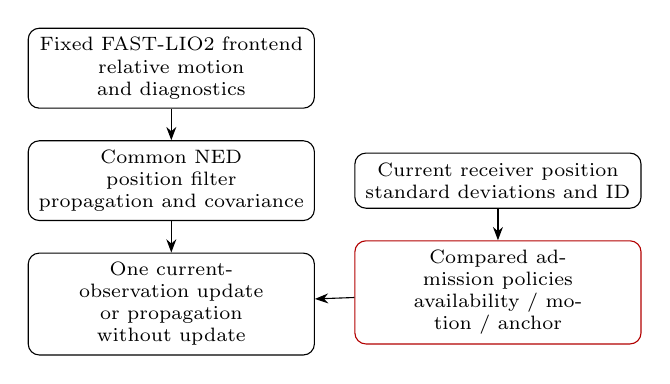
\begin{tikzpicture}[node distance=4mm,every node/.style={draw,rounded corners,font=\scriptsize,align=center,text width=34mm,minimum height=7mm},>=Stealth]
\node (lio) {Fixed FAST-LIO2 frontend\\relative motion and diagnostics};
\node[below=of lio] (prop) {Common NED position filter\\propagation and covariance};
\node[right=5mm of prop] (gnss) {Current receiver position\\standard deviations and ID};
\node[below=of gnss,draw=red!70!black] (manage) {Compared admission policies\\availability / motion / anchor};
\node[below=of prop] (update) {One current-observation update\\or propagation without update};
\draw[->] (lio)--(prop);\draw[->] (prop)--(update);\draw[->] (gnss)--(manage);\draw[->] (manage)--(update);
\end{tikzpicture}
\caption{Executed framework. Only the admission policy varies. Reference states initialize the declared common condition and support offline evaluation; they never enter the manager. KF-GINS remains an independent comparator.}
\label{fig:framework}
\end{figure}
The state is position $p\in\mathbb{R}^{3}$ in NED, with a common initial alignment $A$. For LIO displacement $\Delta\ell_k$,
\begin{align}
 p_k^-&=p_{k-1}^++A\Delta\ell_k,\\
 P_k^-&=P_{k-1}^++\operatorname{diag}(1,1,4)q_k,\\
 q_k&=0.001\Delta t+0.001\|\Delta\ell_k\|.
\end{align}
The coefficients have units $\mathrm{m^2/s}$ and $\mathrm{m^2/m}$. The antenna observation is $z_k=p_k+R_{NB,k}b+v_k$, with FRD lever arm $b=[0,-0.07,-0.365]^\top$ m. Receiver NED standard deviations are floored at $[1,1,2]$ m before squaring to form covariance $R_k$. For an admitted observation,
\begin{align}
 r_k&=z_k-p_k^--R_{NB,k}b,\\
 K_k&=P_k^-(P_k^-+\bar R_k)^{-1},\\
 p_k^+&=p_k^-+K_kr_k,
\end{align}
with Joseph covariance update and policy-inflated $\bar R_k$. Every original receiver ID is consumed once, including rejected observations. Monitoring differences and historical anchors are not independent position measurements.

\subsection{Motion and Historical Anchor}
With receiver position $z$ and independent LIO antenna position $a$, a five-second window checks
\begin{equation}
 d_{ik}=(z_k-z_i)-(a_k-a_i),\quad
 s_{ik}=d_{ik,xy}^{\top}(R_{k,xy}+R_{i,xy}+q_{ik}I)^{-1}d_{ik,xy}.
\end{equation}
The existing P-r03 policy requires an engineering score at most four for two seconds when a motion qualification applies. This score is not a calibrated chi-square test. Gaps greater than 1.5 s clear the monitoring window. An availability shadow policy isolates an anomaly or a GNSS gap greater than two seconds, with a two-second minimum wait and a covariance multiplier initially 15, relaxing over 15 s.

A historical anchor stores the latest raw GNSS observation that was admitted in NORMAL state with valid local diagnostics, acceptable motion score and nominal innovation, continuously qualified for five seconds. During outage recovery it compares
\begin{equation}
 e_k=z_k-\{z_a+(a_k-a_a)\}
\end{equation}
against receiver covariance plus accumulated process covariance. Its horizontal score limit is four. Only an actual GNSS gap activates this anchor check; isolation freezes anchor promotion. Invalid local evidence falls back to the mature availability policy and is logged as unresolved, not as proof of sensor correctness. The two cached interpolation endpoints must have at least 100 effective points and mean absolute plane residual at most 0.2 m for local health eligibility.

This policy cannot distinguish all LIO drift from GNSS bias. A stale or biased anchor can veto useful GNSS; fallback can admit injected observations. There is no bias-state estimation, optimized heading update, or integrity guarantee. The fixed implementation is inherited from R1 rather than revised to fit the R2 results.

\section{Data, Controls, and Evaluation}
\subsection{Inputs and Seen-Data Roles}
The public i2Nav-Robot dataset~\cite{i2nav} supplies AT128 LiDAR, ADIS16465 increments, F9P receiver positions, and an MM/INS reference for building00 and parking00. We verified all 16 supplied raw files against their R1 digests and both bag digests against the official listing. Upstream commits are fixed: i2Nav-Robot at \texttt{2ffdca6d}, its baseline adaptation at \texttt{6c602f8d}, and KF-GINS at \texttt{8291a93e}. Exact hashes, compatibility/logging patches and the reused rootless Noetic runtime are archived.

All policies share the same initialization, cache, covariance, lever arm and observed GNSS timeline within a comparison. The common initial condition reads one explicitly declared reference state and a receiver observation. Later reference values are used only offline. The local NED geodetic origin was not available; errors are initialization-conditioned, not a no-prior absolute WGS84 result. The reference shares AT128 sensing through MM/INS and is not independent of all frontend sensing.

The two building00 frontend caches have identical pose times and verified bag/binary identities, yet their local positions differ by 3.6013 m in 3D RMS. We use the predetermined primary cache and retain the second as a paired sensitivity analysis. They are not independent repeated-route samples. building01 was selected prospectively using documentation only, but its five required raw files remained unavailable. Its performance was never opened. The available analysis archive explicitly does not authorize a new-route opening without complete input identities and a pushed scientific freeze.

\subsection{Fixed Matched Controls}
B2 is LIO propagation without GNSS; B3 is direct position fusion; B4 is the R1-selected NIS gate at 100; B5 is Huber weighting at 2.5; B6 adds the matched availability wait and recovery covariance protection. Clock2/5/10/15/30/60/90 disable the motion and anchor veto while retaining the same availability foundation and covariance policy. The number is qualification duration, not total latency: the five-second monitoring window adds time, producing clean admission delays of 7/10/15/20/35/65/95 s. Clock2 exactly equals the time-only ablation and is counted once.

We also expose the three stricter NIS thresholds already screened in R1: 11.3449, 16.2662 and 30. They were registered as fixed fairness diagnostics before their R2 replays, with no parking-based selection. P-no-motion equals B6; P-no-anchor removes the historical anchor; P-no-decay removes recovery covariance decay. These give 19 distinct named policies. There was no additional mechanism revision or broad parameter search.

\subsection{Events, Clocks, and Coverage}
At fixed offsets 150/450/750 s, with north/east/northeast injection directions, we retain seven event categories and a natural case. Categories are a single 3-m jump, clustered 10-m jumps, 30-s and 60-s observation deletions followed by unmodified data, 30-s deletions followed by 3-m or 10-m biases held for 90 s, and a 10-m ramp. Each category has three fixed events. The primary pair is the 30-s deletion with unmodified return versus the 10-m biased return. ``Unmodified'' does not mean error-free GNSS.

$t_{return}$ is the measurement time of the first actually present observation after deletion; $t_{admit}$ is the first logged \texttt{accepted=true} update. State transitions are insufficient. Admission is censored at a fixed 180-s horizon. We report its measurement-time delay and separately the conservative cache-availability bound; neither is measured live receiver-arrival latency. Offline error recovery is error below 3 m sustained for 5 s within 90 s. Error can already satisfy this condition before any returned GNSS update.

The primary clean service budget is 15 s, inclusive in measurement time. Sensitivity budgets are 5/10/30/60/90 s. Normal cost is natural-case horizontal RMSE no greater than the best frozen B4/B5/B6 value plus $\max(2\%,0.05\,\mathrm{m})$. Every policy appears in full tables regardless of eligibility. Clock10 lies exactly on the measurement-time boundary; its conservative availability bound can exceed 15 s and is separately retained.

Every event is evaluated on the same full 10-Hz expected grid over 10/30/60/90/180 s after return. Event RMSE is averaged equally across the three events, rather than pooling successful samples. A partial window retains its expected count and cannot silently yield a complete RMSE. Injected-row acceptance is counted over the exact artificial bias interval with the denominator retained. This is exposure to injected data, not a probability of a real GNSS fault or a calibrated harm metric.

\section{Results}
\begin{table*}[t]\centering\small
\caption{Complete primary building00 comparison, all 19 policies. RMSE is horizontal, meters; clean delay is maximum actual-update delay across three events, seconds. Exposure is accepted injected rows out of270. Q indicates both the declared natural-cost and inclusive15-s clean service gates. C180 is right-censored admission, not zero latency. All windows have complete expected-grid coverage.}\label{tab:primary}
\begin{tabular}{lrrrrrrc}\toprule
Policy & Natural & Clean delay & Clean90 & Bias90 & Bias180 & Exposure & Q\\\midrule
LIO only & 3.446 & C180 & 1.773 & 1.773 & 2.556 & 0/270 & no \\
Direct fusion & 2.561 & 0.000 & 2.182 & 8.371 & 6.971 & 270/270 & yes \\
NIS100 & 2.561 & 0.000 & 2.182 & 8.371 & 6.971 & 270/270 & yes \\
Huber2.5 & 2.538 & 0.000 & 2.142 & 7.645 & 6.613 & 270/270 & yes \\
Availability B6 & 2.587 & 2.000 & 2.265 & 5.780 & 5.567 & 254/270 & yes \\
NIS11.3449 & 3.185 & 0.000 & 2.095 & 3.653 & 4.279 & 115/270 & no \\
NIS16.2662 & 3.164 & 0.000 & 2.140 & 3.700 & 4.224 & 121/270 & no \\
NIS30 & 2.621 & 0.000 & 2.182 & 3.908 & 3.898 & 127/270 & no \\
Clock2 & 2.587 & 7.000 & 2.313 & 5.558 & 5.429 & 243/270 & yes \\
Clock5 & 2.587 & 10.000 & 2.316 & 5.490 & 5.386 & 234/270 & yes \\
Clock10 & 2.587 & 15.000 & 2.319 & 5.361 & 5.306 & 219/270 & yes \\
Clock15 & 2.587 & 20.000 & 2.321 & 4.899 & 4.967 & 202/270 & no \\
Clock30 & 2.587 & 35.000 & 2.309 & 4.427 & 4.634 & 161/270 & no \\
Clock60 & 2.587 & 65.000 & 2.449 & 2.838 & 3.044 & 73/270 & no \\
Clock90 & 2.587 & 95.000 & 2.509 & 2.510 & 2.411 & 0/270 & no \\
P-r03 & 2.585 & 7.000 & 2.236 & 3.022 & 2.976 & 68/270 & yes \\
P-no-motion & 2.587 & 2.000 & 2.265 & 5.780 & 5.567 & 254/270 & yes \\
P-no-anchor & 2.585 & 7.000 & 2.248 & 5.489 & 5.611 & 237/270 & yes \\
P-no-decay & 2.528 & 7.000 & 2.162 & 3.059 & 2.968 & 68/270 & yes \\
\bottomrule\end{tabular}\end{table*}
\begin{table*}[t]\centering\small
\caption{All controls and ablations on the second building cache and already-seen parking00. Both use the same19 policies and complete coverage. Latencies match Table~\ref{tab:primary}; Q is independently calculated against each cache/route natural cap. Neither column is a new independent R2 test.}\label{tab:other}
\begin{tabular}{lrrrrrrrr}\toprule
 & \multicolumn{4}{c}{Building00 sensitivity cache} & \multicolumn{4}{c}{Parking00 seen historical route}\\
Policy & Natural & Bias90 & Exposure & Q & Natural & Bias90 & Exposure & Q\\\midrule
LIO only & 1.238 & 0.696 & 0/270 & no & 2.356 & 2.226 & 0/270 & no \\
Direct fusion & 2.227 & 8.374 & 270/270 & no & 2.362 & 7.015 & 270/270 & yes \\
NIS100 & 2.227 & 8.374 & 270/270 & no & 2.362 & 3.091 & 162/270 & yes \\
Huber2.5 & 2.154 & 7.660 & 270/270 & no & 2.362 & 6.426 & 270/270 & yes \\
Availability B6 & 2.070 & 5.654 & 252/270 & yes & 2.362 & 4.478 & 254/270 & yes \\
NIS11.3449 & 2.048 & 3.530 & 114/270 & yes & 2.362 & 2.164 & 116/270 & yes \\
NIS16.2662 & 2.104 & 3.545 & 120/270 & yes & 2.362 & 2.128 & 117/270 & yes \\
NIS30 & 2.157 & 3.856 & 129/270 & no & 2.362 & 2.023 & 119/270 & yes \\
Clock2 & 2.070 & 5.480 & 243/270 & yes & 2.362 & 4.395 & 243/270 & yes \\
Clock5 & 2.070 & 5.412 & 234/270 & yes & 2.362 & 4.374 & 234/270 & yes \\
Clock10 & 2.070 & 5.288 & 219/270 & yes & 2.362 & 4.116 & 217/270 & yes \\
Clock15 & 2.070 & 4.827 & 202/270 & no & 2.362 & 3.758 & 202/270 & no \\
Clock30 & 2.070 & 4.365 & 161/270 & no & 2.362 & 3.403 & 161/270 & no \\
Clock60 & 2.070 & 2.542 & 71/270 & no & 2.362 & 2.521 & 75/270 & no \\
Clock90 & 2.070 & 2.085 & 0/270 & no & 2.362 & 2.298 & 0/270 & no \\
P-r03 & 2.070 & 2.884 & 66/270 & yes & 2.362 & 2.290 & 108/270 & yes \\
P-no-motion & 2.070 & 5.654 & 252/270 & yes & 2.362 & 4.478 & 254/270 & yes \\
P-no-anchor & 2.070 & 5.439 & 237/270 & yes & 2.362 & 4.395 & 243/270 & yes \\
P-no-decay & 2.139 & 2.908 & 66/270 & no & 2.362 & 2.259 & 108/270 & yes \\
\bottomrule\end{tabular}\end{table*}

\begin{figure*}[t]\centering
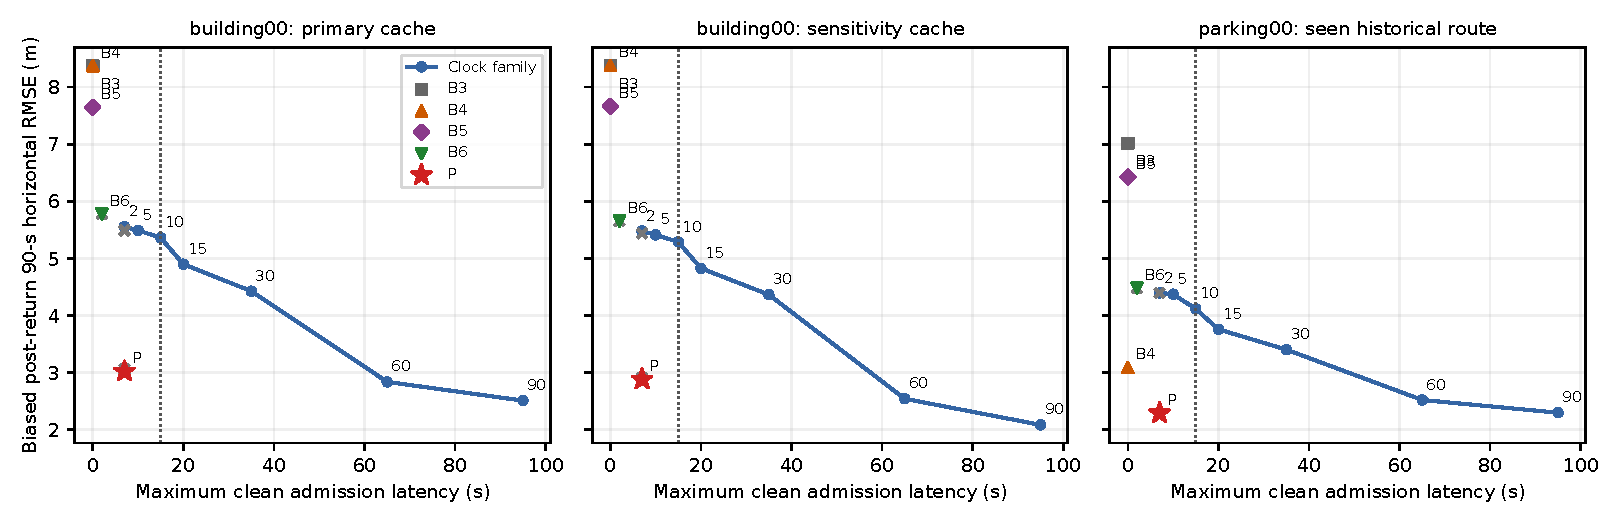
\includegraphics[width=\textwidth]{figures/latency_error_tradeoff.pdf}
\caption{Core policy latency--error tradeoff on all three seen caches. Numbers on the connected Clock curve are qualification durations. The dotted line is the 15-s clean measurement-time budget. Gray crosses are ablations. Full point files and Tables~\ref{tab:primary}--\ref{tab:other} retain all stricter NIS diagnostics and censored B2 outcomes; lower error outside the budget remains evidence.}
\label{fig:tradeoff}\end{figure*}

\subsection{Completeness and Building-Route Tradeoff}
The matrix contains 456 matched policy--cache--case pairs and 1,197 fixed event records. Of these, 296 pairs are inherited and 160 are additional cached controls; there is no old-route frontend redeployment. All whole-route and event windows have full coverage. Recomputed inherited whole-route RMSE equals its archived value exactly. A separate checker, which does not import the main evaluator, verifies 6,441 error values, all 1,197 admission clocks and exposure counts, with maximum absolute error difference $4.44\times10^{-16}$ m. Original 64 regression tests and nine added metric tests pass. Failed checker/harness attempts are retained alongside their corrected executions.

On the primary building cache, P admits unmodified returned GNSS in 7 s for all three events and has natural RMSE 2.5847 m, within the 2.5890-m cap. Its biased post90 RMSE is 3.0222 m, versus Clock10's 5.3611 m, and its accepted injected count is 68/270 versus 219/270. However, Huber has lower clean post90 error, 2.1419 versus 2.2361 m. Stricter NIS30 obtains biased error 3.9082 m and natural error 2.6212 m, exceeding the stated cap by about 0.0322 m; this result is retained. A 5\% natural-cost allowance would include it, while P still has lower biased error on this cache. This sensitivity does not replace the registered gate.

The second building cache preserves the conditional biased-return trend: P has 2.8837-m post90 error and 66/270 accepted injected rows. The strictest NIS control has 3.5304 m and 114/270 and satisfies its natural-cost cap. Yet P's clean error, 1.8854 m, exceeds B6's 1.8601 m. Thus the result is an explicit tradeoff rather than improvement in every dimension.

\subsection{Stronger Long Waits and Parking Counterexample}
Clock90 admits clean data after 95 s and accepts no biased rows during the 90-s injection. It obtains lower biased post90 error than P on both building caches: 2.5098 versus 3.0222 m and 2.0854 versus 2.8837 m. The extended 180-s results also favor Clock90 on those caches. The earlier R1 conclusion that P does not establish added gain under unrestricted aggregate error therefore remains valid.

The parking route provides a stronger counterexample to a universal method claim. NIS30 has zero clean-admission delay and 2.0234-m biased post90 error, compared with P's 7 s and 2.2901 m. P accepts eleven fewer injected rows, 108 versus 119, but that count does not establish lower actual harm. We report the stricter NIS result directly rather than limiting the parking comparison to the weaker selected NIS100 baseline.

An offline antenna-error check further finds that injected bias reduces the declared initialization-conditioned receiver error for 16 of 270 building rows and 46 of 270 parking rows. Consequently exposure counts must be interpreted alongside actual trajectory error, receiver covariance and the artificial scenario. They cannot be converted into field fault-detection accuracy.

\subsection{Ablations and Event-Level Failures}
Removing the anchor raises primary building biased post90 error from 3.0222 to 5.4893 m; removing motion yields B6's 5.7798 m. This supports a conditional role of the already-existing anchor on this route. It does not establish a new R2 method increment. Removing covariance decay gives slightly higher building post90 error, but lower parking error, 2.2587 versus 2.2901 m, and fails the second-cache natural-cost gate. Decay is not a uniformly necessary contribution.

\begin{figure}[t]\centering
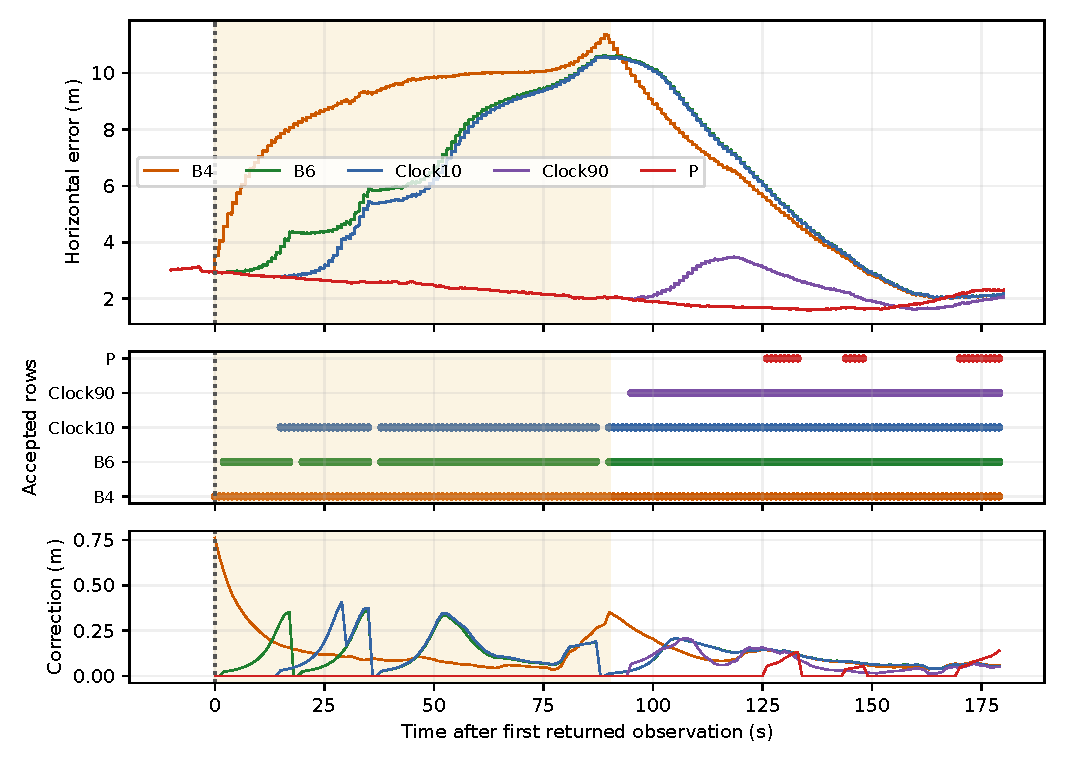
\includegraphics[width=\columnwidth]{figures/first_registered_bias_event.pdf}
\caption{First registered primary biased-return event, selected by order. Shading covers the 90-s injection. Error, actually accepted observation rows, and update corrections are distinct. P's first admitted update is at 126 s; its clean seven-second latency does not describe this biased event.}
\label{fig:event}\end{figure}
Event-level results expose failure that a macro statistic hides. P admits no injected rows in the first primary biased event and first updates at 126 s, 36 s after bias removal. In the third event it first updates at 25 s and accepts 65 of 90 injected rows. The second cache similarly has a 124-s first-event admission and 63 injected acceptances in the third. In parking event zero, P admits 82/90 injected rows. These records are not censored away or replaced by favorable examples. The first-event time series in Fig.~\ref{fig:event} follows the fixed event order rather than the largest winning margin.

\section{Discussion and Scientific Judgment}
The data support an empirical latency--error tension and a constrained building-route tradeoff. They do not support superiority over every simple control, a calibrated probability of erroneous GNSS admission, an independent R2 effect, or novelty of motion-based recovery. The unchanged policy uses current and historical sensor information causally, but its anchor shares correlated GNSS/LIO evidence and its score lacks a rigorous independence model. The classifier cannot resolve observation-equivalent local drift and GNSS bias.

The five-second Clock window makes the comparison foundation explicit; a different fixed-wait implementation could expose a different curve. Our benchmark covers the declared existing controls rather than all possible thresholds or adaptive waiting rules. The normal-cost constraint is a stated application gate and excludes some strong strict-NIS outcomes on the primary cache; those outcomes remain fully visible. Within-route events are few, fixed and correlated, so we present descriptive paired results without an IID significance claim.

The frontend repeatability issue remains unresolved. Identical verified bag/binary identities, pose timestamps and 12,440 output rows do not guarantee identical estimates; the first difference above $10^{-8}$ m begins near 80 s, and the maximum difference reaches 9.7876 m. The two runs also differ in clock availability and EOF handling. The available logs do not prove a concurrency root cause. Unflagged numerical LIO reset is not detected by the current interface; a retained synthetic test demonstrates that a large jump can be propagated. Fixed alignment, common known initialization, shared reference sensing and synthetic bias all restrict transferability.

Timing scopes remain separate. The previously measured primary frontend processing mean/P95 are 17.32/22.77 ms per scan; these exclude GNSS backend and deployed transport. Python cached replay times are not end-to-end online timing. The transferred native KF-GINS parking configuration produced 76.56-m horizontal RMSE in R1; this is a configuration-transfer failure, not KF-GINS's best accuracy and is not used as a main improvement denominator.

Because building01 remained unavailable, a new-route scientific freeze and first independent performance evaluation could not be completed. The present review package is a complete seen-data study with an explicit missing-input condition. Its scientific status is narrower than a method paper; human authors should assess whether an empirical submission is suitable after independent validation and venue checks.

\section{Conclusion}
GNSS admission time, injected-observation exposure and trajectory error are distinct endpoints. Complete matched waits show why lower error can accompany delayed clean correction. The retained motion-and-anchor policy offers a building-route tradeoff under the declared service budget, while stricter NIS gating is faster and more accurate on seen parking data. No new mechanism was promoted and no independent generalization was established. These boundaries, stronger controls and failure records are part of the result.

\section*{Reproducibility and Review Disclosure}
Exact sources, configurations, hashes, event tables, vector plots and independent checks are retained on the authorized R2 branch of \url{https://github.com/zhoumy0313/lio-gins}. Large sensor files and full trajectory logs remain local; the Git remote is a partial evidence backup. Raw data are not verified as remotely backed up. The i2Nav dataset is used for academic analysis under its stated terms. No authorship, affiliation, funding, copyright agreement or formal submission is asserted. IEEE conference layout is provisional; venue template, anonymity and deadline timezone remain unverified.

OpenAI Codex (GPT-6) assisted executable orchestration, evaluation-script development, evidence organization, manuscript text and plot code throughout this study. Numeric plots are generated from retained data, not synthetic artwork. This assistance is disclosed in Methods through the recorded verification procedure and here for all manuscript sections. Human authors have not yet approved the scientific interpretation or submission; they must verify code, references and wording before adoption.
\bibliographystyle{IEEEtran}
\bibliography{references}
\end{document}
